\documentclass{article}
\usepackage[shortlabels]{enumitem}
\usepackage{amsmath,amsthm,graphicx,hyperref,multirow,longtable,tikz}
\newtheorem{theorem}{Theorem}
\title{TejTeX Integration Document}
\author{Ada Lovelace \and Alan Turing}
\date{2026}
\begin{document}
\maketitle
\begin{abstract}
This document exercises every Phase~4 feature at once.
\end{abstract}

\section{Introduction}\label{sec:intro}
This is \textbf{bold}, \emph{emphasis with \emph{nested} text}, \texttt{code}, \underline{underlined} and \textsc{Small Caps}.
Forward references: Section~\ref{sec:results}, \autoref{fig:chart}, Table~\ref{tab:scores},
Equation~\eqref{eq:euler}, Theorem~\ref{thm:main} and item~\ref{it:deep}.
Read more at \url{https://example.org/tejtex} or \href{https://www.ctan.org}{CTAN}.
An unsafe link stays text: \href{javascript:alert(1)}{do not click}.
A footnote follows.\footnote{The footnote has a label.\label{fn:note}}

\section{Lists}\label{sec:lists}
\begin{enumerate}
\item First step.
\item Second step with a nested list:
  \begin{enumerate}
  \item Inner step.
    \begin{itemize}
    \item A bullet inside.
      \begin{enumerate}
      \item Deep step. \label{it:deep}
      \end{enumerate}
    \end{itemize}
  \end{enumerate}
\item[(x)] Custom label.
\item Third step.
\end{enumerate}
\begin{enumerate}[(a)]
\item Restarted list in another format.
\end{enumerate}
\begin{description}
\item[Term] A description list entry.
\end{description}

\section{Tables}\label{sec:tables}
\begin{table}[h]
\centering
\caption{Scores with merged cells}\label{tab:scores}
\begin{tabular}{|l|c|p{0.4\linewidth}|}
\hline
Group & \multicolumn{2}{c|}{Details} \\
\hline
\multirow{2}{*}{A} & 1 & \begin{itemize}\item listed \item in a cell\end{itemize} \\
 & 2 & 
\includegraphics[width=1cm]{figs/logo.jpg} with an image \\
\hline
B & 3 & Plain text \\
\hline
\end{tabular}
\end{table}

\begin{longtable}{ll}
Number & Description \\
\hline
\endhead
1 & Row 1 of the long table \\
2 & Row 2 of the long table \\
3 & Row 3 of the long table \\
4 & Row 4 of the long table \\
5 & Row 5 of the long table \\
6 & Row 6 of the long table \\
7 & Row 7 of the long table \\
8 & Row 8 of the long table \\
9 & Row 9 of the long table \\
10 & Row 10 of the long table \\
11 & Row 11 of the long table \\
12 & Row 12 of the long table \\
13 & Row 13 of the long table \\
14 & Row 14 of the long table \\
15 & Row 15 of the long table \\
16 & Row 16 of the long table \\
17 & Row 17 of the long table \\
18 & Row 18 of the long table \\
19 & Row 19 of the long table \\
20 & Row 20 of the long table \\
21 & Row 21 of the long table \\
22 & Row 22 of the long table \\
23 & Row 23 of the long table \\
24 & Row 24 of the long table \\
25 & Row 25 of the long table \\
26 & Row 26 of the long table \\
27 & Row 27 of the long table \\
28 & Row 28 of the long table \\
29 & Row 29 of the long table \\
30 & Row 30 of the long table \\
31 & Row 31 of the long table \\
32 & Row 32 of the long table \\
33 & Row 33 of the long table \\
34 & Row 34 of the long table \\
35 & Row 35 of the long table \\
36 & Row 36 of the long table \\
37 & Row 37 of the long table \\
38 & Row 38 of the long table \\
39 & Row 39 of the long table \\
40 & Row 40 of the long table \\
41 & Row 41 of the long table \\
42 & Row 42 of the long table \\
43 & Row 43 of the long table \\
44 & Row 44 of the long table \\
45 & Row 45 of the long table \\
46 & Row 46 of the long table \\
47 & Row 47 of the long table \\
48 & Row 48 of the long table \\
49 & Row 49 of the long table \\
50 & Row 50 of the long table \\
51 & Row 51 of the long table \\
52 & Row 52 of the long table \\
53 & Row 53 of the long table \\
54 & Row 54 of the long table \\
55 & Row 55 of the long table \\
56 & Row 56 of the long table \\
57 & Row 57 of the long table \\
58 & Row 58 of the long table \\
59 & Row 59 of the long table \\
60 & Row 60 of the long table \\
\end{longtable}

\section{Figures}\label{sec:figures}
\begin{figure}[h]
\centering
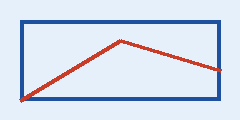
\includegraphics[width=0.5\textwidth]{figs/chart.png}
\caption{A chart}\label{fig:chart}
\end{figure}
The same chart again, inline: 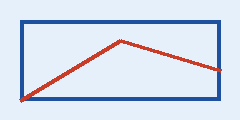
\includegraphics[height=1cm]{figs/chart.png} and
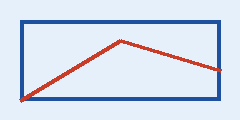
\includegraphics[height=1cm]{figs/chart}.
\begin{figure}[h]
\centering
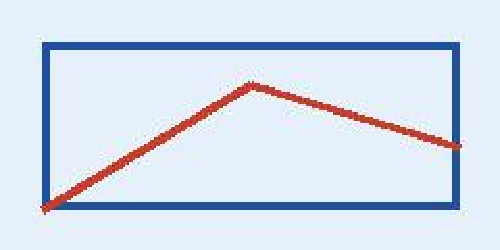
\includegraphics{figs/diagram.pdf}
\caption{A vector diagram}
\end{figure}

\section{Mathematics}\label{sec:math}
\begin{equation}
e^{i\pi} + 1 = 0 \label{eq:euler}
\end{equation}
\begin{align}
a &= b \label{eq:first} \\
c &= d \label{eq:second}
\end{align}
\begin{theorem}[Main result]\label{thm:main}
Every reference in this document resolves.
\end{theorem}

\section{Unsupported content}\label{sec:unsupported}
\begin{tikzpicture}
\draw (0,0) -- (1,1);
\end{tikzpicture}
An unknown command: \unknowncmd{argument}.

\section{Results}\label{sec:results}
Backward references: Section~\ref{sec:intro}, Section~\ref{sec:lists}, Figure~\ref{fig:chart},
Table~\ref{tab:scores}, Equations~\eqref{eq:first} and~\eqref{eq:second}, \autoref{thm:main},
footnote~\ref{fn:note}, \hyperref[sec:tables]{the tables section} and \cite{knuth}.
An undefined reference: \ref{sec:missing}.
\begin{thebibliography}{9}
\bibitem{knuth} D. E. Knuth. The \TeX book. 1984.
\end{thebibliography}
\end{document}
